%! suppress = MissingLabel


\chapter{State of the art}

While the primary focus of this work lies in infrastructure design rather than algorithmic innovation, a brief overview of key prediction algorithms (e.g., AlphaFold) is essential to understand the operational requirements and constraints that the infrastructure must support.


\section{Machine Learning in Protein Structure Prediction}

AlphaFold represents a breakthrough in computational biology, developed by Google DeepMind to predict three--dimensional protein structures with unprecedented accuracy.
This AI system revolutionized the field by achieving near--experimental accuracy in protein structure prediction.

\subsection{Preliminary information}

AlphaFold emerged as the winner of the CASP14 competition in 2020, demonstrating remarkable accuracy in protein structure prediction.
The system leverages deep learning techniques to predict protein structures from amino acid sequences.
AlphaFold 2 represents a significant improvement over previous methods, with a median GDT score exceeding 90 for many targets.
Later AlphaFold 3 extended capabilities to predict protein--protein, protein--nucleic acid, and protein--ligand interactions.
The scientific impact includes accelerating drug discovery, understanding disease mechanisms, and designing novel proteins with specific functions.

\subsection{Algorithm implementation}

AlphaFold implements a novel neural network architecture combining attention mechanisms with structure--based learning.
The algorithm processes protein sequences through multiple specialized neural network blocks.
First, an evolutionary MSA transformer analyzes multiple sequence alignments to capture evolutionary patterns.
Then, a structure module with invariant point attention integrates geometric constraints.
The system iteratively refines predictions through a recycling mechanism that feeds intermediate results back into the network.
Final outputs include 3D atomic coordinates with confidence metrics for each residue.
The implementation balances computational efficiency with prediction accuracy through careful optimization.

\subsection{Program operation overview}

AlphaFold operates in several distinct stages during protein structure prediction, as shown in Figure~\ref{fig:alphafold}.
Initially, it searches sequence databases to build multiple sequence alignments for the target protein.
This first stage requires only CPU resources and involves sequence similarity searches against large databases.
Next, the system processes this data through its neural network architecture to generate initial structure predictions, a stage that exclusively requires GPU resources for efficient tensor operations.
The prediction undergoes multiple refinement cycles, where each iteration improves model quality.
AlphaFold produces five candidate models with associated confidence scores (pLDDT). The deployment involves containerized environments for reproducibility across computing platforms.
Output formats include PDB files for 3D coordinates and additional files containing confidence metrics and model parameters.

\begin{figure}[htbp]
    \centering
    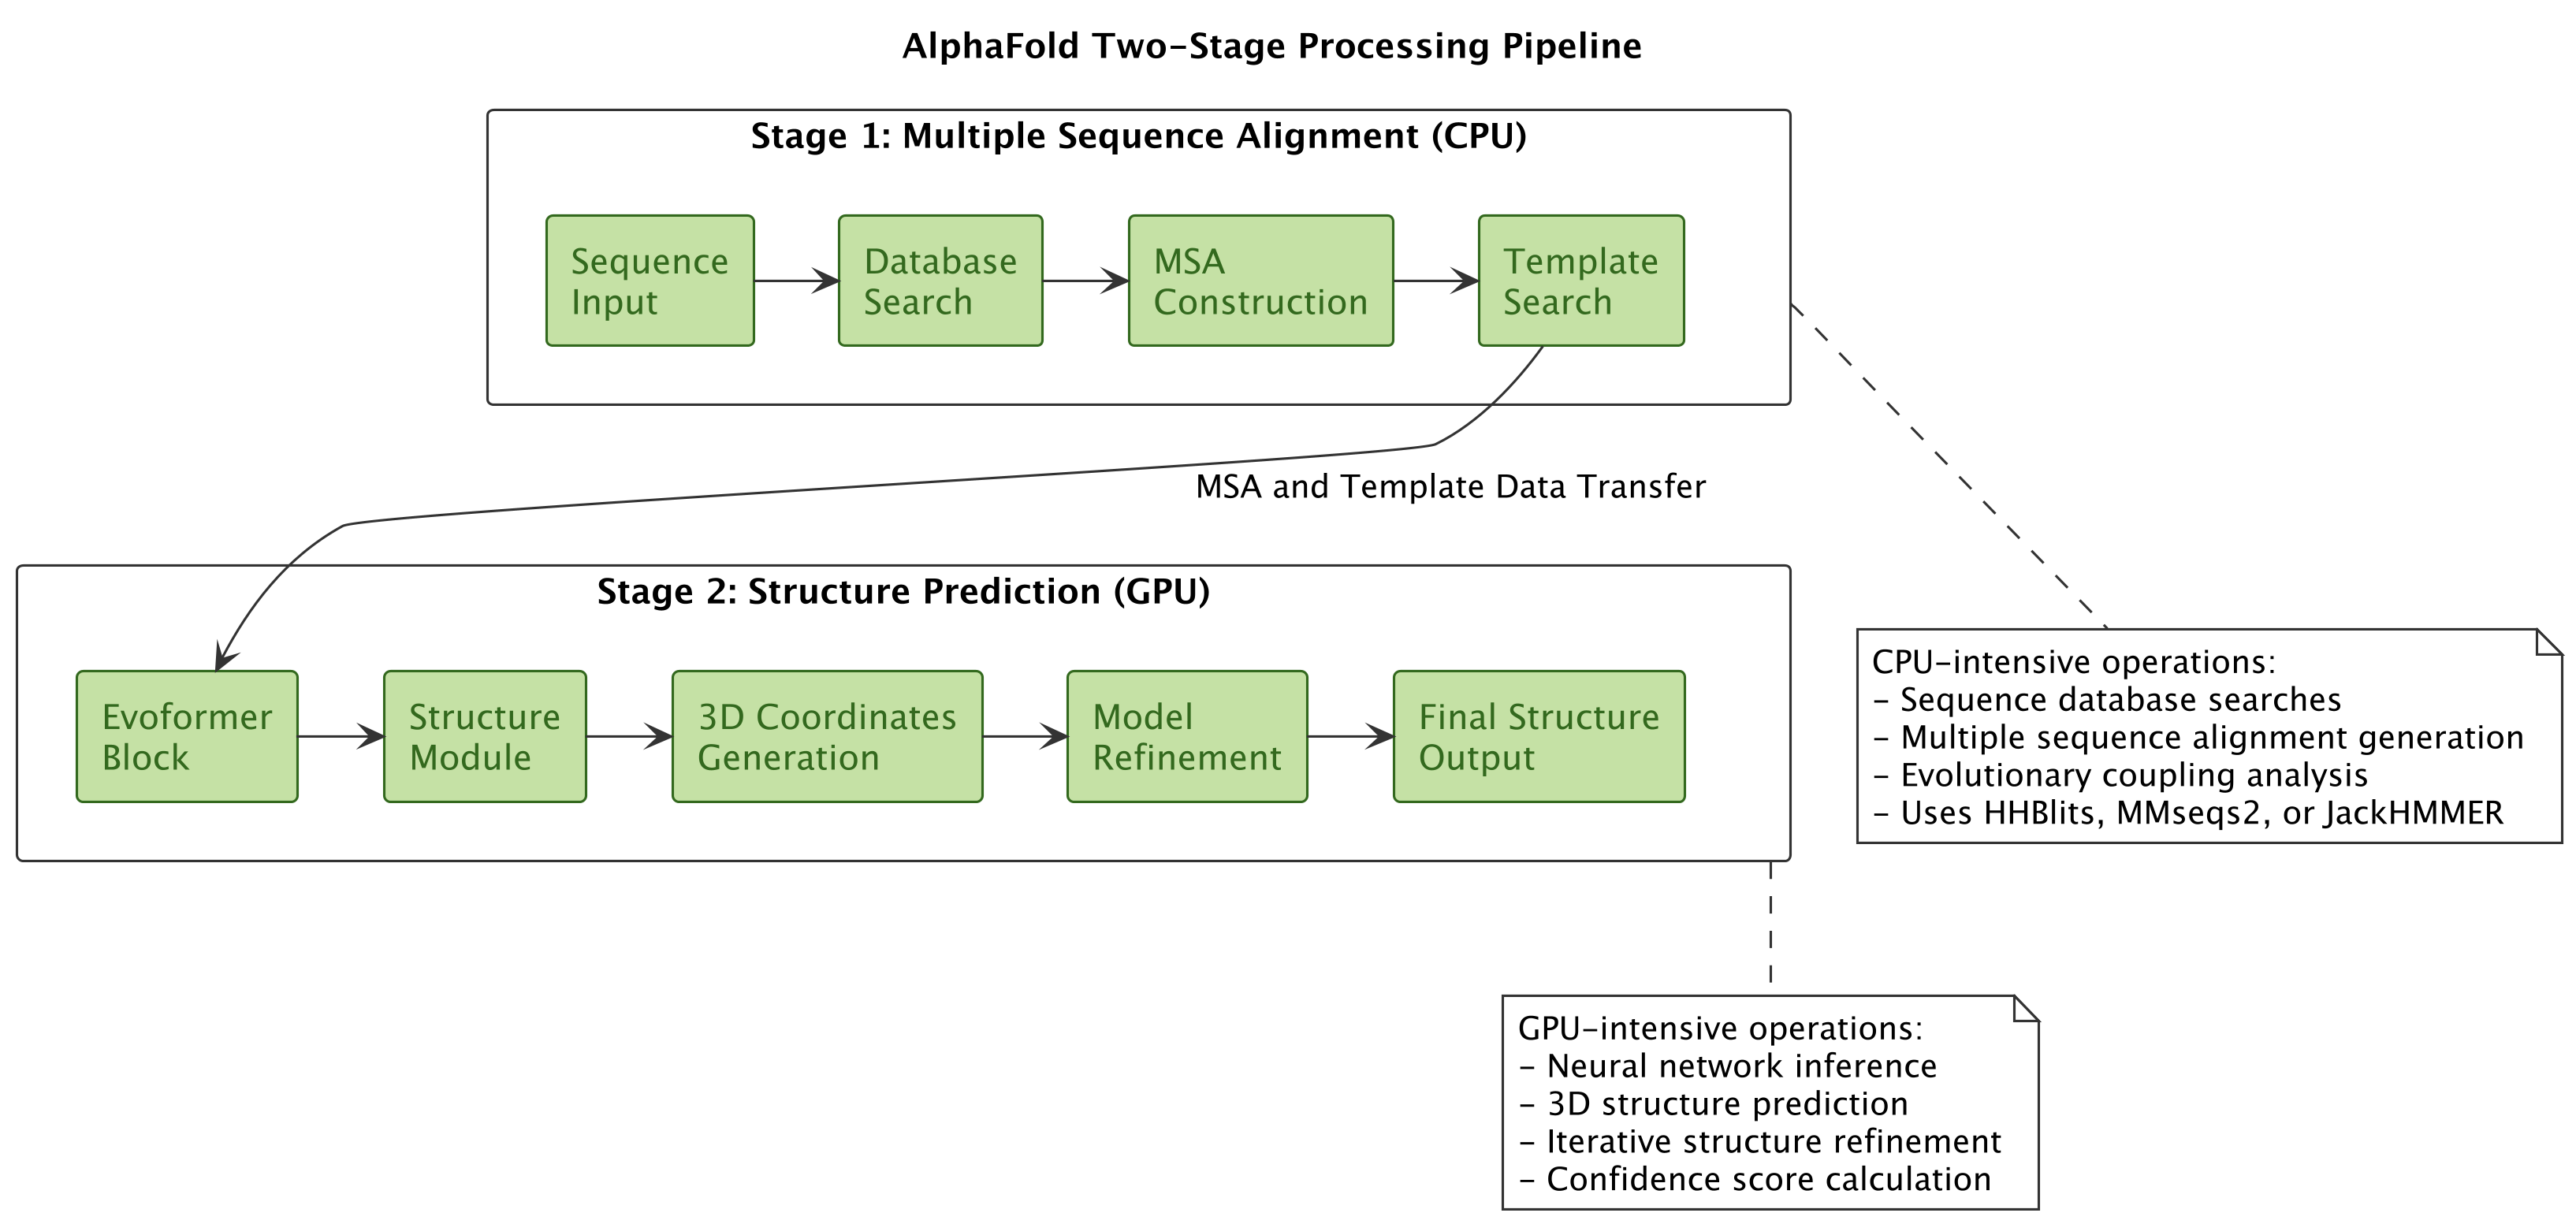
\includegraphics[width=\textwidth]{images/alphafold}
    \caption{AlphaFold 3 computation stages}
    \label{fig:alphafold}
\end{figure}

\subsection{Required computational resources}

AlphaFold demands substantial computational resources for effective operation.
The system requires high--performance GPUs, preferably NVIDIA A100 or similar, with at least 16GB VRAM. Memory requirements range from 16GB for small proteins to 64GB+ for large complexes.
Storage needs include approximately 2TB for reference databases and additional space for output models.
Prediction time varies significantly with protein size and complexity, ranging from 30 minutes for small proteins to several hours for complex structures.
Cloud--based deployments typically cost between $10--$100 per prediction depending on computational requirements.
The high resource demands make AlphaFold particularly suitable for execution in specialized computing environments with access to dedicated hardware accelerators.


\section{Computational clusters in a cloud environment}

\subsection{Kubernetes platform}

Kubernetes is an open--source container orchestration software that automates the deployment, scaling, and management of applications~\cite{kubernetes, container_orchestration}.
It is currently the main solution in the area of computational cluster management.
Kubernetes originates from Google's internal project called Borg, which was released as an open--source project in 2014.

The main goal of Kubernetes is to provide a platform for running applications in a distributed environment.
The system enables automatic management of computational resources in a heterogeneous hardware environment, encompassing different processor architectures and dedicated computational accelerators.
Kubernetes eliminates many manual processes related to deploying and scaling containerized applications.
All cluster components are controlled declaratively.

The Kubernetes architecture is based on a master--worker node model.
The main control component (control plane) manages worker nodes, on which actual applications are run in containers.
Each Kubernetes cluster consists of at least one master node and many worker nodes.
This architecture provides high availability and fault tolerance.

The resource model in Kubernetes is declarative.
Pod is the basic deployment unit in Kubernetes, representing one or more containers that share resources and are always run on the same cluster node.
After loading a configuration file in YAML format, Kubernetes will strive to bring the actual state of the cluster to the state declared in the configuration.
An example of a \texttt{Deployment} resource declaration shown in listing~\ref{lst:kube-deployment} contains comments explaining key elements:

\begin{lstlisting}[language=yaml,caption={Example Deployment declaration in Kubernetes},label={lst:kube-deployment}]
apiVersion: apps/v1
# Kubernetes resource type
kind: Deployment 
metadata:
  name: nginx-deployment
  labels:
    app: nginx
spec:
  # Number of replicas (copies) of the pod to run
  replicas: 3
  # Selector specifying which pods belong to the deployment
  selector:
    matchLabels:
      app: nginx
  # Template defining pod specification
  template:
    metadata:
      labels:
        app: nginx
    spec:
      containers:
      # Container definition to run
      - name: nginx
        image: nginx:1.14.2
        ports:
        - containerPort: 80  # Port to listen on in the container
\end{lstlisting}

Kubernetes introduces an abstraction of the infrastructure layer.
This allows applications to be moved between different cloud providers without modifying code.
The platform supports various runtime environments, from local clusters, through private clouds, to major public cloud providers.

Key capabilities of Kubernetes include:
\begin{itemize}
    \item Automatic application recovery in case of failure,
    \item Load balancing and network traffic distribution,
    \item Automatic horizontal scaling of applications based on a load,
    \item Configuration and secrets management,
    \item Persistent storage management,
    \item Batch execution for batch jobs and computation scheduling.
\end{itemize}

Kubernetes was designed as an extensible platform.
It allows creating custom controllers and operators tailored to specific needs.
This extensibility is key for the KubeFold project, which uses these mechanisms to orchestrate complex protein conformation prediction tasks.

\subsection{Architecture and components of a Kubernetes cluster}

A Kubernetes cluster consists of two main parts: the Control Plane and Worker Nodes, as shown in Figure~\ref{fig:kubernetes-architecture}.
This architecture provides the foundation for running containerized applications like AlphaFold in a distributed environment~\cite{kubernetes}.

The Control Plane contains components that manage the entire cluster and store its state:
\begin{itemize}
    \item \textbf{kube--api--server} -- the access point to the cluster, handling all API requests and providing the interface for communication,
    \item \textbf{etcd} -- a key--value database storing the entire cluster state, serving as the persistent storage for all cluster configuration,
    \item \textbf{kube--scheduler} -- responsible for assigning workloads to nodes based on resource requirements and constraints,
    \item \textbf{kube--controller--manager} -- supervises the cluster state, ensuring it matches the declared configuration by running controller processes,
    \item \textbf{cloud--controller--manager} -- integrates the cluster with cloud provider infrastructure, managing cloud--specific resources.
\end{itemize}

Worker Nodes run actual workloads in the form of containers.
Each worker node contains:
\begin{itemize}
    \item \textbf{kubelet} -- an agent managing containers on the node, ensuring they are running and healthy,
    \item \textbf{kube--proxy} -- handling network traffic and ensuring routing between services across the cluster,
    \item \textbf{Pods} -- the basic deployment units containing one or more containers that share networking and storage resources.
\end{itemize}

As described earlier in the Kubernetes Platform section, the system defines higher--level abstractions such as \texttt{Deployment} or \texttt{StatefulSet}.
These enable declarative application management through configuration files in YAML format.
The Service resource provides a stable access point to a group of Pods, abstracting the underlying infrastructure changes.

The cluster uses a plugin system to extend functionality.
This includes storage, network, or monitoring drivers.
Particularly important for the KubeFold project are Custom Resource Definitions, which allow adding custom resource types as discussed in the Cluster Operator section.

The Kubernetes architecture ensures high availability, scalability, and fault tolerance required for computational tasks like protein structure prediction.
Components can be duplicated across nodes to prevent single points of failure.
The system automatically responds to failures by restarting and relocating applications, maintaining the desired state of the cluster.

\begin{figure}[htbp]
    \centering
    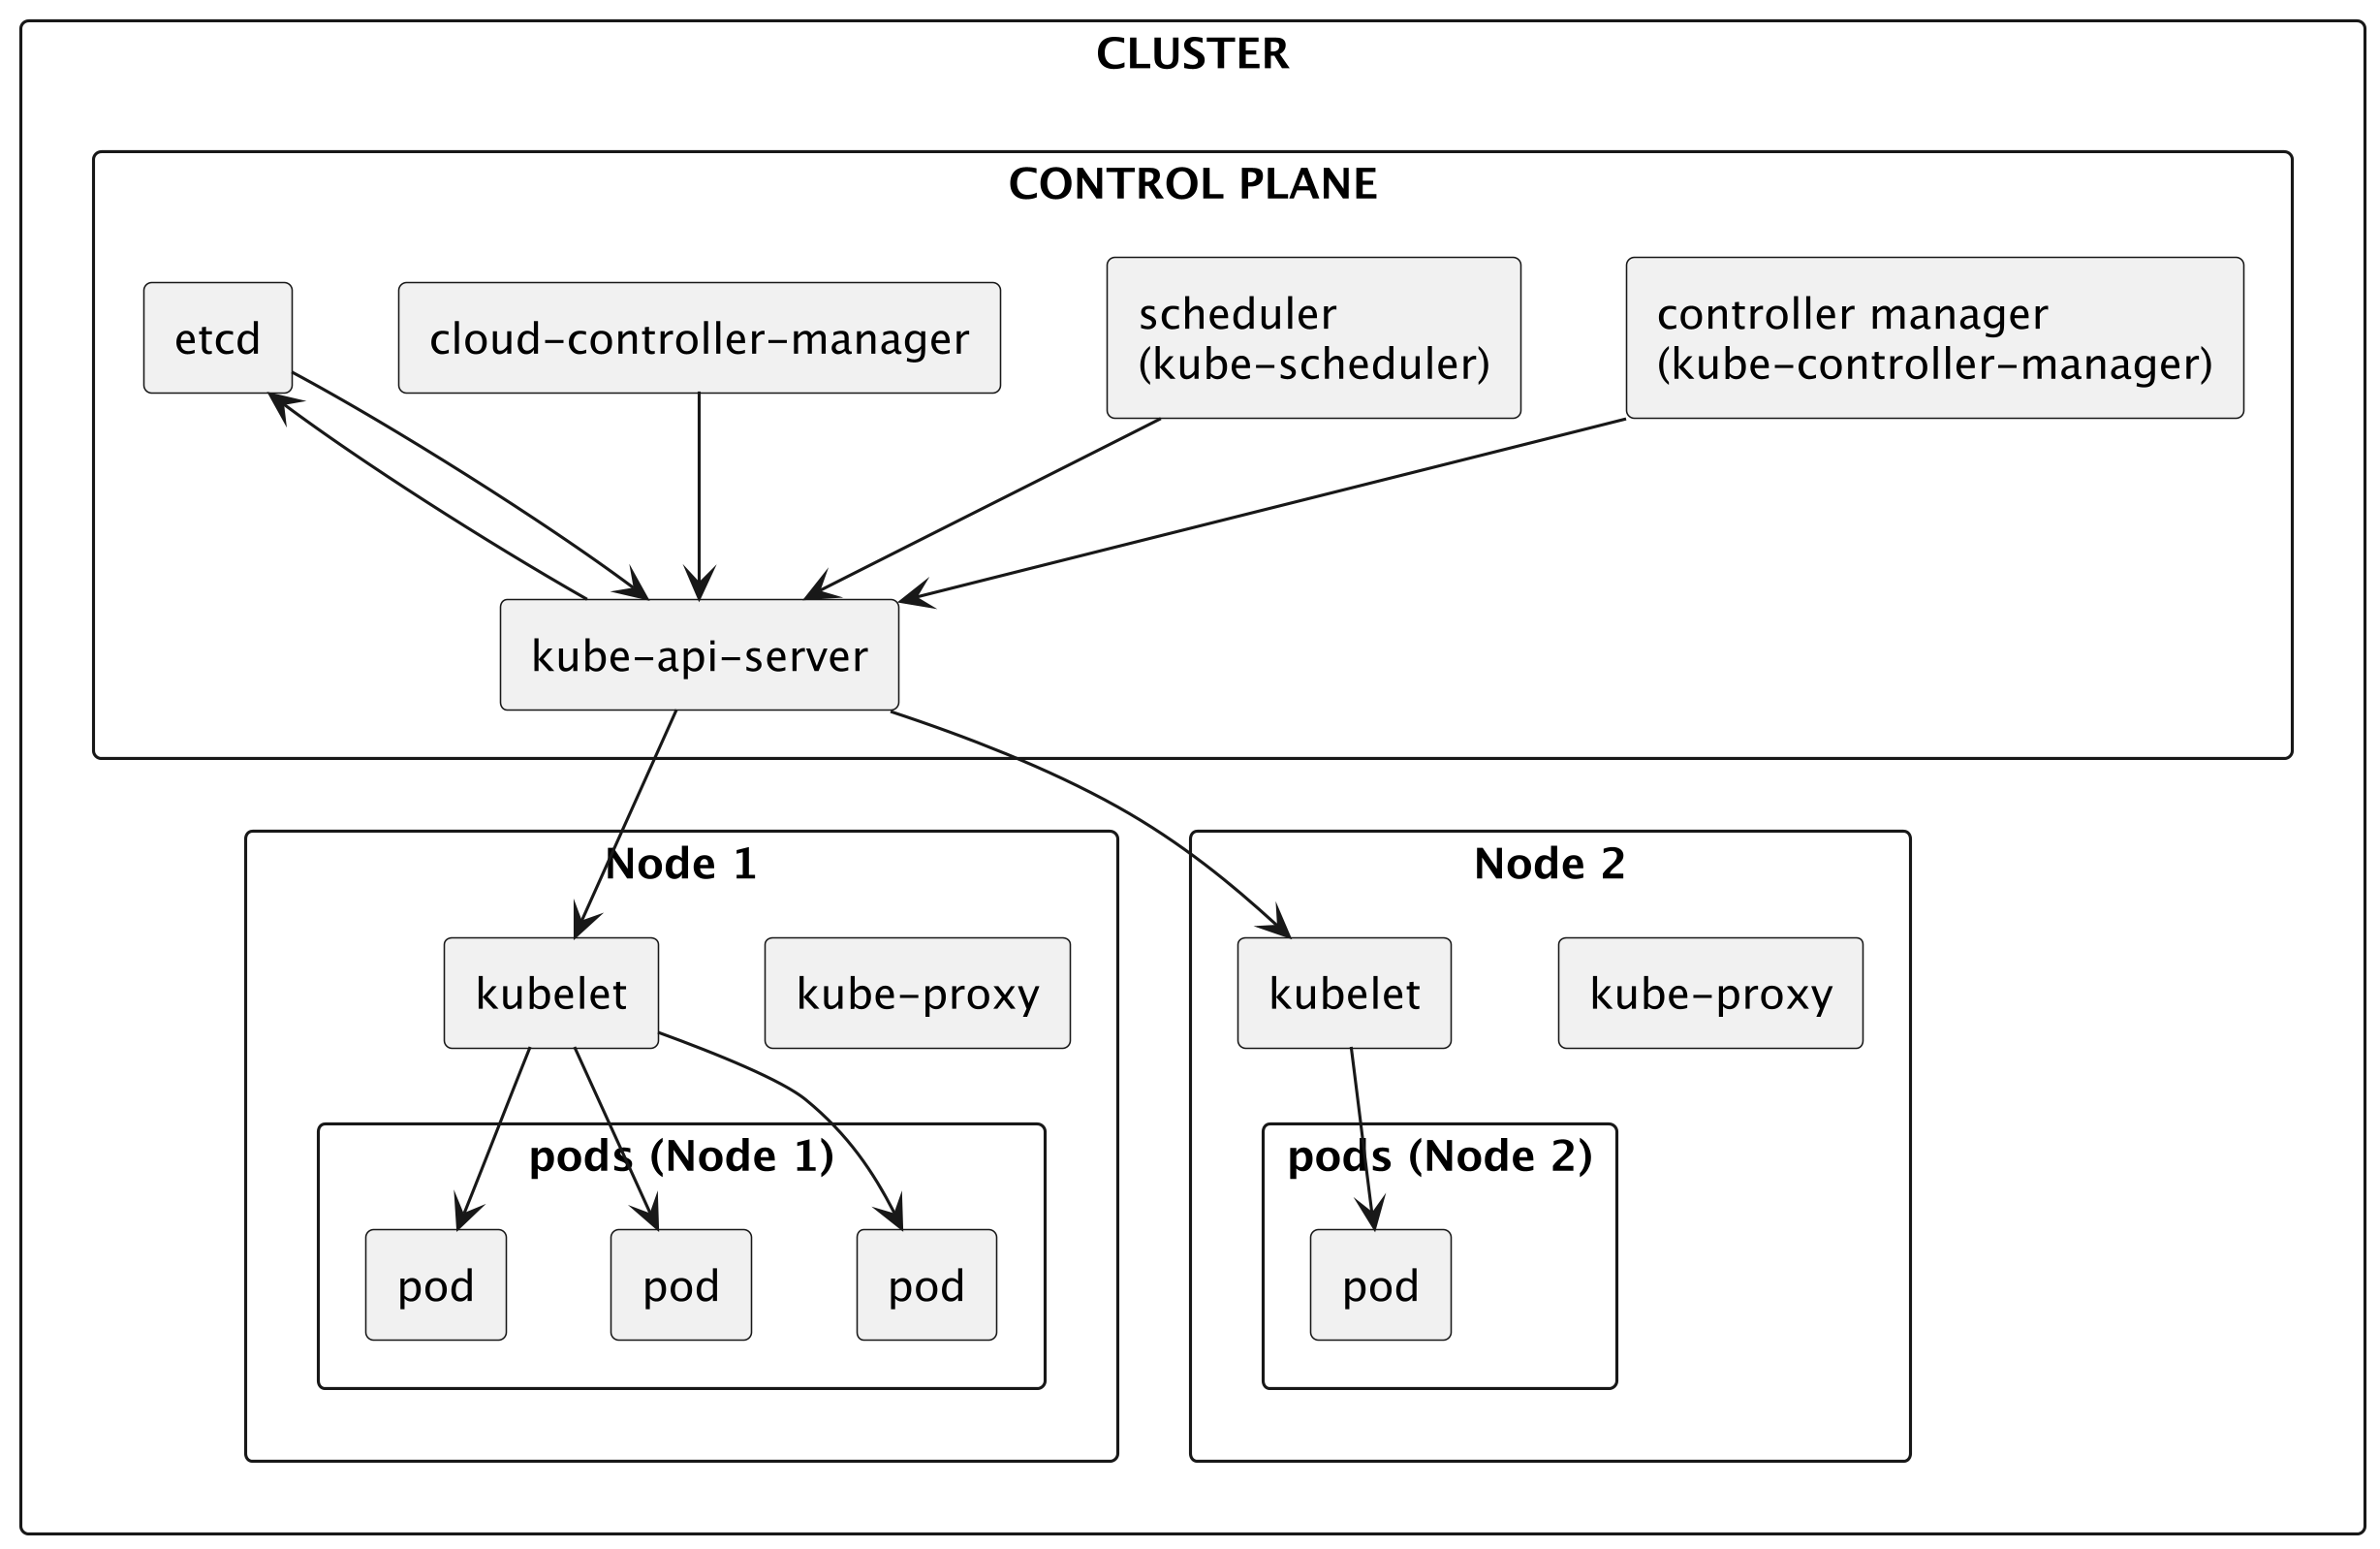
\includegraphics[width=\textwidth]{images/kubernetes}
    \caption{Kubernetes cluster architecture showing Control Plane components (kube--api--server, etcd, scheduler, controller manager, cloud--controller--manager) and Worker Nodes containing kubelet, kube--proxy, and pods. The diagram illustrates the communication between the control plane and worker nodes, with the cloud provider API interface for external resource management.}
    \label{fig:kubernetes-architecture}
\end{figure}

\subsection{Available resources in the computational cluster}
Kubernetes platform defines basic resource types used to manage applications in a computational cluster.
Each resource type serves a specific role and can be configured by administrators and applications.

\subsubsection{Pod}
Pod is the basic deployment unit in a Kubernetes cluster.
It represents a process executing an application along with its execution context.
A Pod contains one or more containers sharing network space and storage resources.
Listing~\ref{lst:pod-example} shows an example definition of a Pod with an application server and an attached data volume.

\begin{lstlisting}[language=yaml,caption={Example Pod definition},label={lst:pod-example}]
apiVersion: v1
kind: Pod
metadata:
  name: web-server
  labels:
    app: web
spec:
  containers:
  - name: nginx
    image: nginx:latest
    resources:
      limits:
        memory: "128Mi"
        cpu: "500m"
    volumeMounts:
    - name: www-data
      mountPath: /usr/share/nginx/html
  volumes:
  - name: www-data
    persistentVolumeClaim:
      claimName: web-content
\end{lstlisting}

\subsubsection{Job}
Job represents a computational task with a finite execution time.
This resource guarantees successful execution of a specified number of Pods.
In case of a computational node failure, the Job automatically creates a new Pod instance.
Listing~\ref{lst:job-example} shows an example of a Job performing batch file conversion.

\begin{lstlisting}[language=yaml,caption={Example Job definition},label={lst:job-example}]
apiVersion: batch/v1
kind: Job
metadata:
  name: batch-convert
spec:
  template:
    spec:
      containers:
      - name: converter
        image: imagemagick:latest
        command: ["convert"]
        args: ["*.jpg", "-resize", "800x600", "output/"]
      restartPolicy: Never
  backoffLimit: 4
\end{lstlisting}

\subsubsection{PersistentVolume}
PersistentVolume defines a persistent storage volume in the cluster.
It is independent of the Pod lifecycle and stores data that must survive cluster restarts.
Listing~\ref{lst:pv-example} shows the definition of a volume using the NFS file system.

\begin{lstlisting}[language=yaml,caption={Example PersistentVolume definition},label={lst:pv-example}]
apiVersion: v1
kind: PersistentVolume
metadata:
  name: nfs-volume
spec:
  capacity:
    storage: 100Gi
  accessModes:
    - ReadWriteMany
  persistentVolumeReclaimPolicy: Retain
  nfs:
    server: nfs-server.example.com
    path: "/shared"
\end{lstlisting}

\subsubsection{PersistentVolumeClaim}
PersistentVolumeClaim is a request for allocation of storage resources~\cite{k8s_persistent_volumes}.
It defines requirements regarding the size and access mode for the volume.
Listing~\ref{lst:pvc-example} shows an example request for creating a 10GB volume.

\begin{lstlisting}[language=yaml,caption={Example PersistentVolumeClaim definition},label={lst:pvc-example}]
apiVersion: v1
kind: PersistentVolumeClaim
metadata:
  name: web-content
spec:
  accessModes:
    - ReadWriteMany
  resources:
    requests:
      storage: 10Gi
  storageClassName: standard
\end{lstlisting}

\subsubsection{StorageClass}
StorageClass describes a storage class available in the cluster.
It defines the provider and configuration parameters for volumes.
Listing~\ref{lst:sc-example} shows the definition of a standard storage class for SSD disks.

\begin{lstlisting}[language=yaml,caption={Example StorageClass definition},label={lst:sc-example}]
apiVersion: storage.k8s.io/v1
kind: StorageClass
metadata:
  name: fast-storage
provisioner: kubernetes.io/aws-ebs
parameters:
  type: gp3
  iopsPerGB: "5000"
  encrypted: "true"
reclaimPolicy: Delete
allowVolumeExpansion: true
\end{lstlisting}

\subsection{Volume allocation mechanism}
Kubernetes uses a complex mechanism for dynamic allocation of storage resources.
When an application creates a PersistentVolumeClaim, the system checks the storage class (StorageClass) declared in it.
Based on this, it activates the appropriate driver that creates a physical volume in the infrastructure.
The newly created PersistentVolume is then automatically linked to the claim.
Thanks to this mechanism, a cluster administrator can define different storage classes, and users can use them without knowing the technical details of the infrastructure.
The system guarantees that the volume will exist as long as the claim associated with it exists.
After deleting a PersistentVolumeClaim, the fate of the volume depends on the defined reclaim policy -- it can be automatically deleted or preserved for reuse.

\subsection{Kubernetes clusters in the cloud}

Kubernetes clusters in a cloud environment represent a natural evolution of computational platforms.
The cloud offers dynamic resource allocation and integration with services such as data stores or monitoring systems.
Geographic distribution ensures high availability, and automatic backup mechanisms protect against data loss.
Advanced access control systems guarantee the security of data and applications.

Public cloud providers offer managed Kubernetes services that automate most administrative tasks.
This includes cluster creation and configuration, component updates, and infrastructure state monitoring.
Thanks to this, teams can focus on application development instead of infrastructure maintenance.

\subsection{Managed Kubernetes service in Amazon Web Services}\label{subsec:aws-eks}

Amazon Elastic Kubernetes Service (EKS) is a comprehensive solution for running Kubernetes clusters in the AWS cloud~\cite{amazon_eks}.
The service automatically manages control node updates, certificates, and network configuration.
Integration with AWS services simplifies creating solutions using data stores or notification systems.

In the context of the KubeFold project, access to instances equipped with graphics cards and integration with the FSx for Lustre file system are of key importance.
EKS enables automatic scaling of the node group depending on demand, which translates into cost optimization.

Using Kubernetes clusters in the cloud brings significant benefits for computational projects.
Elimination of costs for maintaining own infrastructure and access to specialized hardware without the need to purchase allow for flexible budget management.
The billing model based on actual resource consumption works particularly well in the case of computations with varying intensity, such as protein conformation prediction.
Automatic recovery mechanisms after failure and global availability ensure reliability and high--quality services.
This combination of features makes cloud Kubernetes clusters an optimal environment for modern scientific applications.

\subsection{Lustre volumes}\label{subsec:lustre-volumes}

Lustre is a distributed file system, created by Cluster File Systems in 2003~\cite{lustre_fs}.
This system was designed for high--performance computing clusters.
Currently, the development of Lustre is managed by the OpenSFS (Open Scalable File Systems) organization.

The Lustre file system consists of several main components, as shown in Figure~\ref{fig:lustre-arch}:
\begin{itemize}
    \item Metadata servers (MDS) -- store information about the file system structure, directories, and permissions,
    \item Object storage servers (OSS) -- responsible for storing actual data and handling input/output operations,
    \item Clients -- nodes that mount the file system and use it,
    \item Metadata target devices (MDT) -- store metadata on block devices,
    \item Object storage targets (OST) -- store file data on block devices.
\end{itemize}

\begin{figure}[htbp]
    \centering
    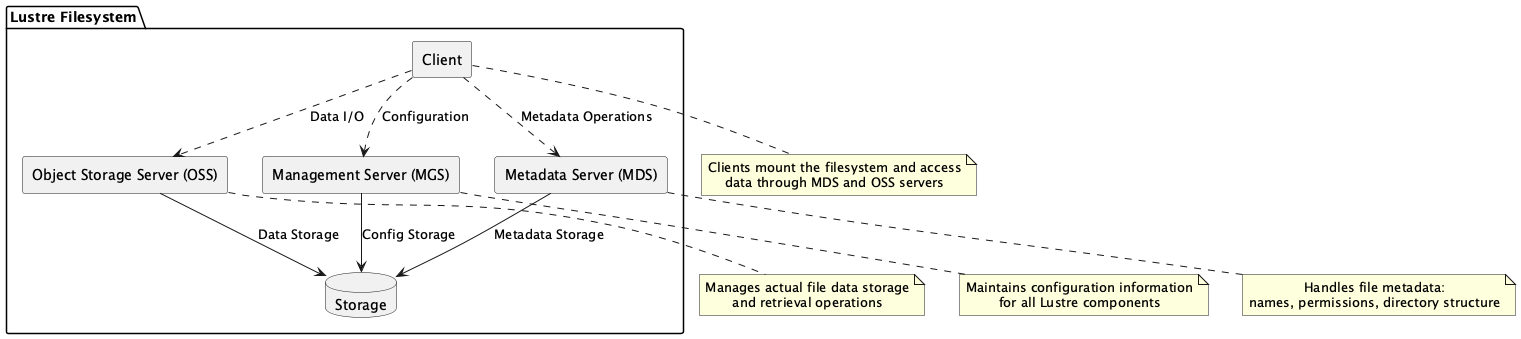
\includegraphics[width=\textwidth]{images/lustre}
    \caption{Lustre distributed file system architecture showing the relationships between metadata servers, object storage servers, and clients.}
    \label{fig:lustre-arch}
\end{figure}

The Lustre architecture is based on the separation of metadata from actual data.
Metadata servers deal exclusively with operations on directory structure and permissions.
Object servers handle operations on the file data itself.
Such separation allows for optimization of both types of operations independently.

Lustre ensures very high performance through parallel input/output operations.
The system enables simultaneous access to the same files from multiple cluster nodes.
A single Lustre file system can serve tens of thousands of clients simultaneously.
The system's throughput scales linearly with the addition of more object servers.

Main features of the Lustre file system:
\begin{itemize}
    \item High scalability -- ability to handle petabytes of data and thousands of nodes,
    \item High throughput -- ability to achieve throughput in the terabit per second range,
    \item Cache coherence -- guarantee of data consistency between all clients,
    \item Fault tolerance -- ability to work despite failure of individual components,
    \item Support for multiple access protocols -- POSIX, MPI--IO, HDFS\@.
\end{itemize}

In the KubeFold project, Lustre is a key component for storing protein databases.
Its architecture ensures high throughput and low latency when accessing data.
The system allows simultaneous access to files from multiple cluster nodes performing calculations.
This makes it possible to parallel process data by multiple instances of the AlphaFold algorithm.

Lustre is widely used in computing centers around the world.
It is used in supercomputers from the TOP500 list.
The system works particularly well in scientific computing, where processing huge datasets is required.
Examples of applications include physical simulations, climate modeling, and genomic calculations.

\subsection{Amazon FSx for Lustre}\label{subsec:amazon-fsx-for-lustre}

Amazon FSx for Lustre is a fully managed service that provides high--performance Lustre file systems in the AWS cloud~\cite{aws_fsx}.
The service automatically handles all the complexity of setting up and managing Lustre infrastructure, including server provisioning, software configuration, and system maintenance.

\begin{figure}[htbp]
    \centering
    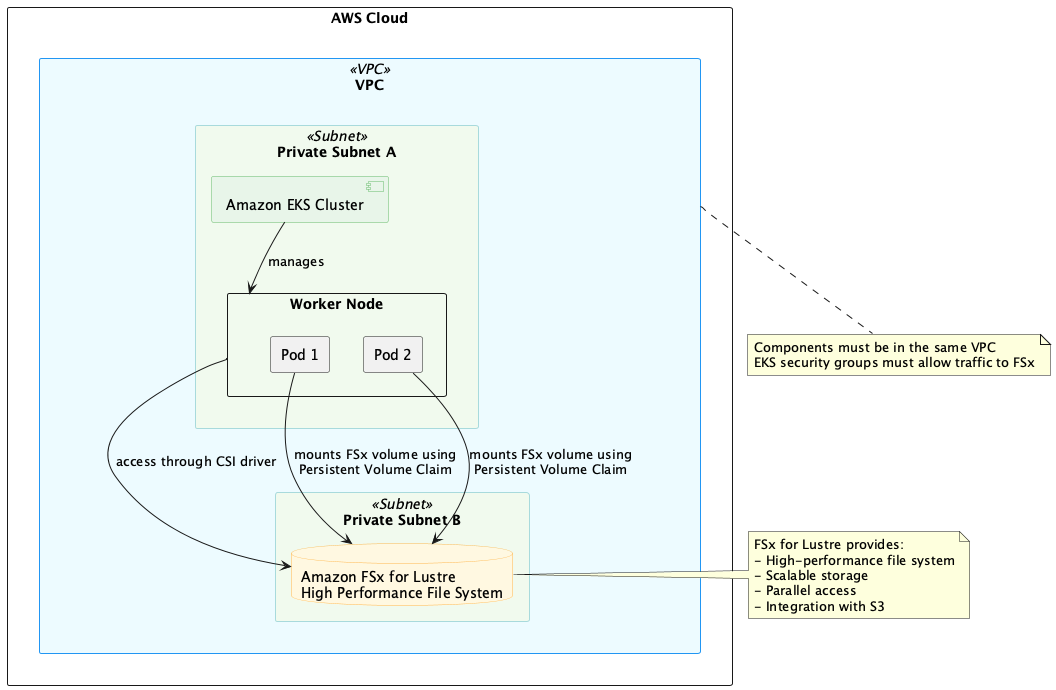
\includegraphics[width=\textwidth]{images/fsx}
    \caption{Architecture diagram showing EKS cluster connection to FSx for Lustre volume}
    \label{fig:fsx-architecture}
\end{figure}

Key features of FSx for Lustre include:
\begin{itemize}
    \item Automatic scaling of storage capacity and performance,
    \item Built--in data protection with automatic backups,
    \item Native integration with AWS services like EC2 and EKS,
    \item Support for multiple storage deployment options (scratch, persistent),
    \item Throughput capacity up to hundreds of GB per second.
\end{itemize}

The service offers two deployment types:
\begin{itemize}
    \item Scratch -- optimized for temporary storage and shorter--term processing, with higher performance,
    \item Persistent -- designed for longer--term storage with data replication and backup support.
\end{itemize}

In the context of the KubeFold project, FSx for Lustre provides high--performance storage for AlphaFold databases and computation results, as shown in Figure~\ref{fig:fsx-architecture}.
The automatic management and scaling capabilities simplify operations while maintaining the performance required for protein structure predictions.

\subsection{Amazon S3 object storage}\label{subsec:amazon-s3-object-storage}

Amazon Simple Storage Service (S3) is a cloud object storage service~\cite{aws_s3}.
It provides virtually unlimited disk space with guaranteed availability of 99.999999999\%.
It is an industry standard for cloud data storage.

The basic organizational unit in S3 are buckets.
Each bucket has a globally unique name and can store any number of objects.
Objects are identified by keys, which can contain slash characters to create a hierarchical structure.

S3 has become the standard for data storage in cloud applications.
Most modern cloud solutions provide integration with this system.
Tool providers often implement S3 support as the first choice for integrations with data stores.

The service provides a REST API interface and libraries for many programming languages.
Authentication uses digital signatures or temporary credentials.
Access control is based on IAM policies and ACL lists.
These standard mechanisms are widely used in the cloud ecosystem.

S3 provides full integration with other AWS services.
It is commonly used as storage for backups, a place to store artifacts, or the target location for computation results.
Its reliability and scalability make it the primary choice for applications requiring persistent data storage.

\subsection{AWS End User Messaging Service}\label{subsec:amazon-sns}

AWS End User Messaging is a service that enables sending SMS messages to end users~\cite{aws_messaging}.
It uses the Amazon Simple Notification Service (SNS) infrastructure to deliver messages.

The service offers the following capabilities:
\begin{itemize}
    \item sending individual SMS messages,
    \item sending group messages,
    \item monitoring delivery status,
    \item managing sending limits,
    \item automatic shortening of long messages.
\end{itemize}

The system handles two types of SMS messages:
\begin{itemize}
    \item Promotional -- optimized for cost,
    \item Transactional -- optimized for delivery reliability.
\end{itemize}

The service provides global reach through cooperation with multiple mobile operators.
Messages can be sent to over 200 countries and territories.
SNS automatically selects the best route for message delivery.

The service billing is based on the number of messages sent.
The price depends on the target country and the chosen message type.
The system offers cost control mechanisms through setting monthly spending limits.

Integration with the service is done through the REST API interface or SDK sets available for popular programming languages.
The service also provides detailed event logs and metrics available in Amazon CloudWatch.

The KubeFold platform uses AWS End User Messaging to notify researchers about the completion of protein structure calculations by the AlphaFold algorithm.
The system sends SMS messages containing information about task status and links to results in S3 storage.


\section{Cluster operator concept}

A Kubernetes operator is a program that extends cluster capabilities with automatic management of complex applications~\cite{k8s_operators}.
An operator automates tasks that would normally require manual intervention from a system administrator.

Custom Resource Definitions (CRDs) are the fundamental building blocks of an operator.
These resources define new types of objects that can be managed within a Kubernetes cluster.
The operator continuously monitors the state of these resources and performs necessary actions to keep the system running as expected.

The operator automates typical administrative tasks such as:
\begin{itemize}
    \item Installing and updating applications,
    \item Creating and restoring backups,
    \item Detecting and fixing failures,
    \item Modifying application settings.
\end{itemize}

Operators are particularly effective at managing stateful applications like databases and messaging systems.
In such cases, the operator automatically performs complex operations that typically require specialized knowledge.

An operator consists of two main parts: custom resource definitions and a management program.
The management program continuously compares the current system state with the desired state and implements necessary changes.

\subsection{Cluster operator architecture}

A Kubernetes operator follows a control loop pattern called the reconciliation loop.
This pattern continuously monitors the cluster state and makes adjustments to maintain the desired configuration.
The operator consists of several key components working together to manage custom resources.

The core components of an operator architecture include:

\begin{itemize}
    \item Custom Resource Definition (CRD) -- Defines the schema and validation rules for custom resources,
    \item Controller -- Implements the business logic and reconciliation loop,
    \item Client -- Interfaces with the Kubernetes API to read and modify resources,
    \item Cache -- Maintains an in--memory copy of watched resources for efficiency,
    \item Work Queue -- Buffers reconciliation requests to handle them sequentially.
\end{itemize}

The reconciliation loop follows these main steps:
\begin{enumerate}
    \item Watch for changes to custom resources and related Kubernetes objects,
    \item Compare current state with desired state specified in the custom resource,
    \item Calculate what changes are needed to reach desired state,
    \item Apply the necessary changes through the Kubernetes API,
    \item Update status of the custom resource.
\end{enumerate}

Figure~\ref{fig:kubernetes-operator-flow} illustrates the typical interaction flow between components in a Kubernetes operator:

\begin{figure}[htbp]
    \centering
    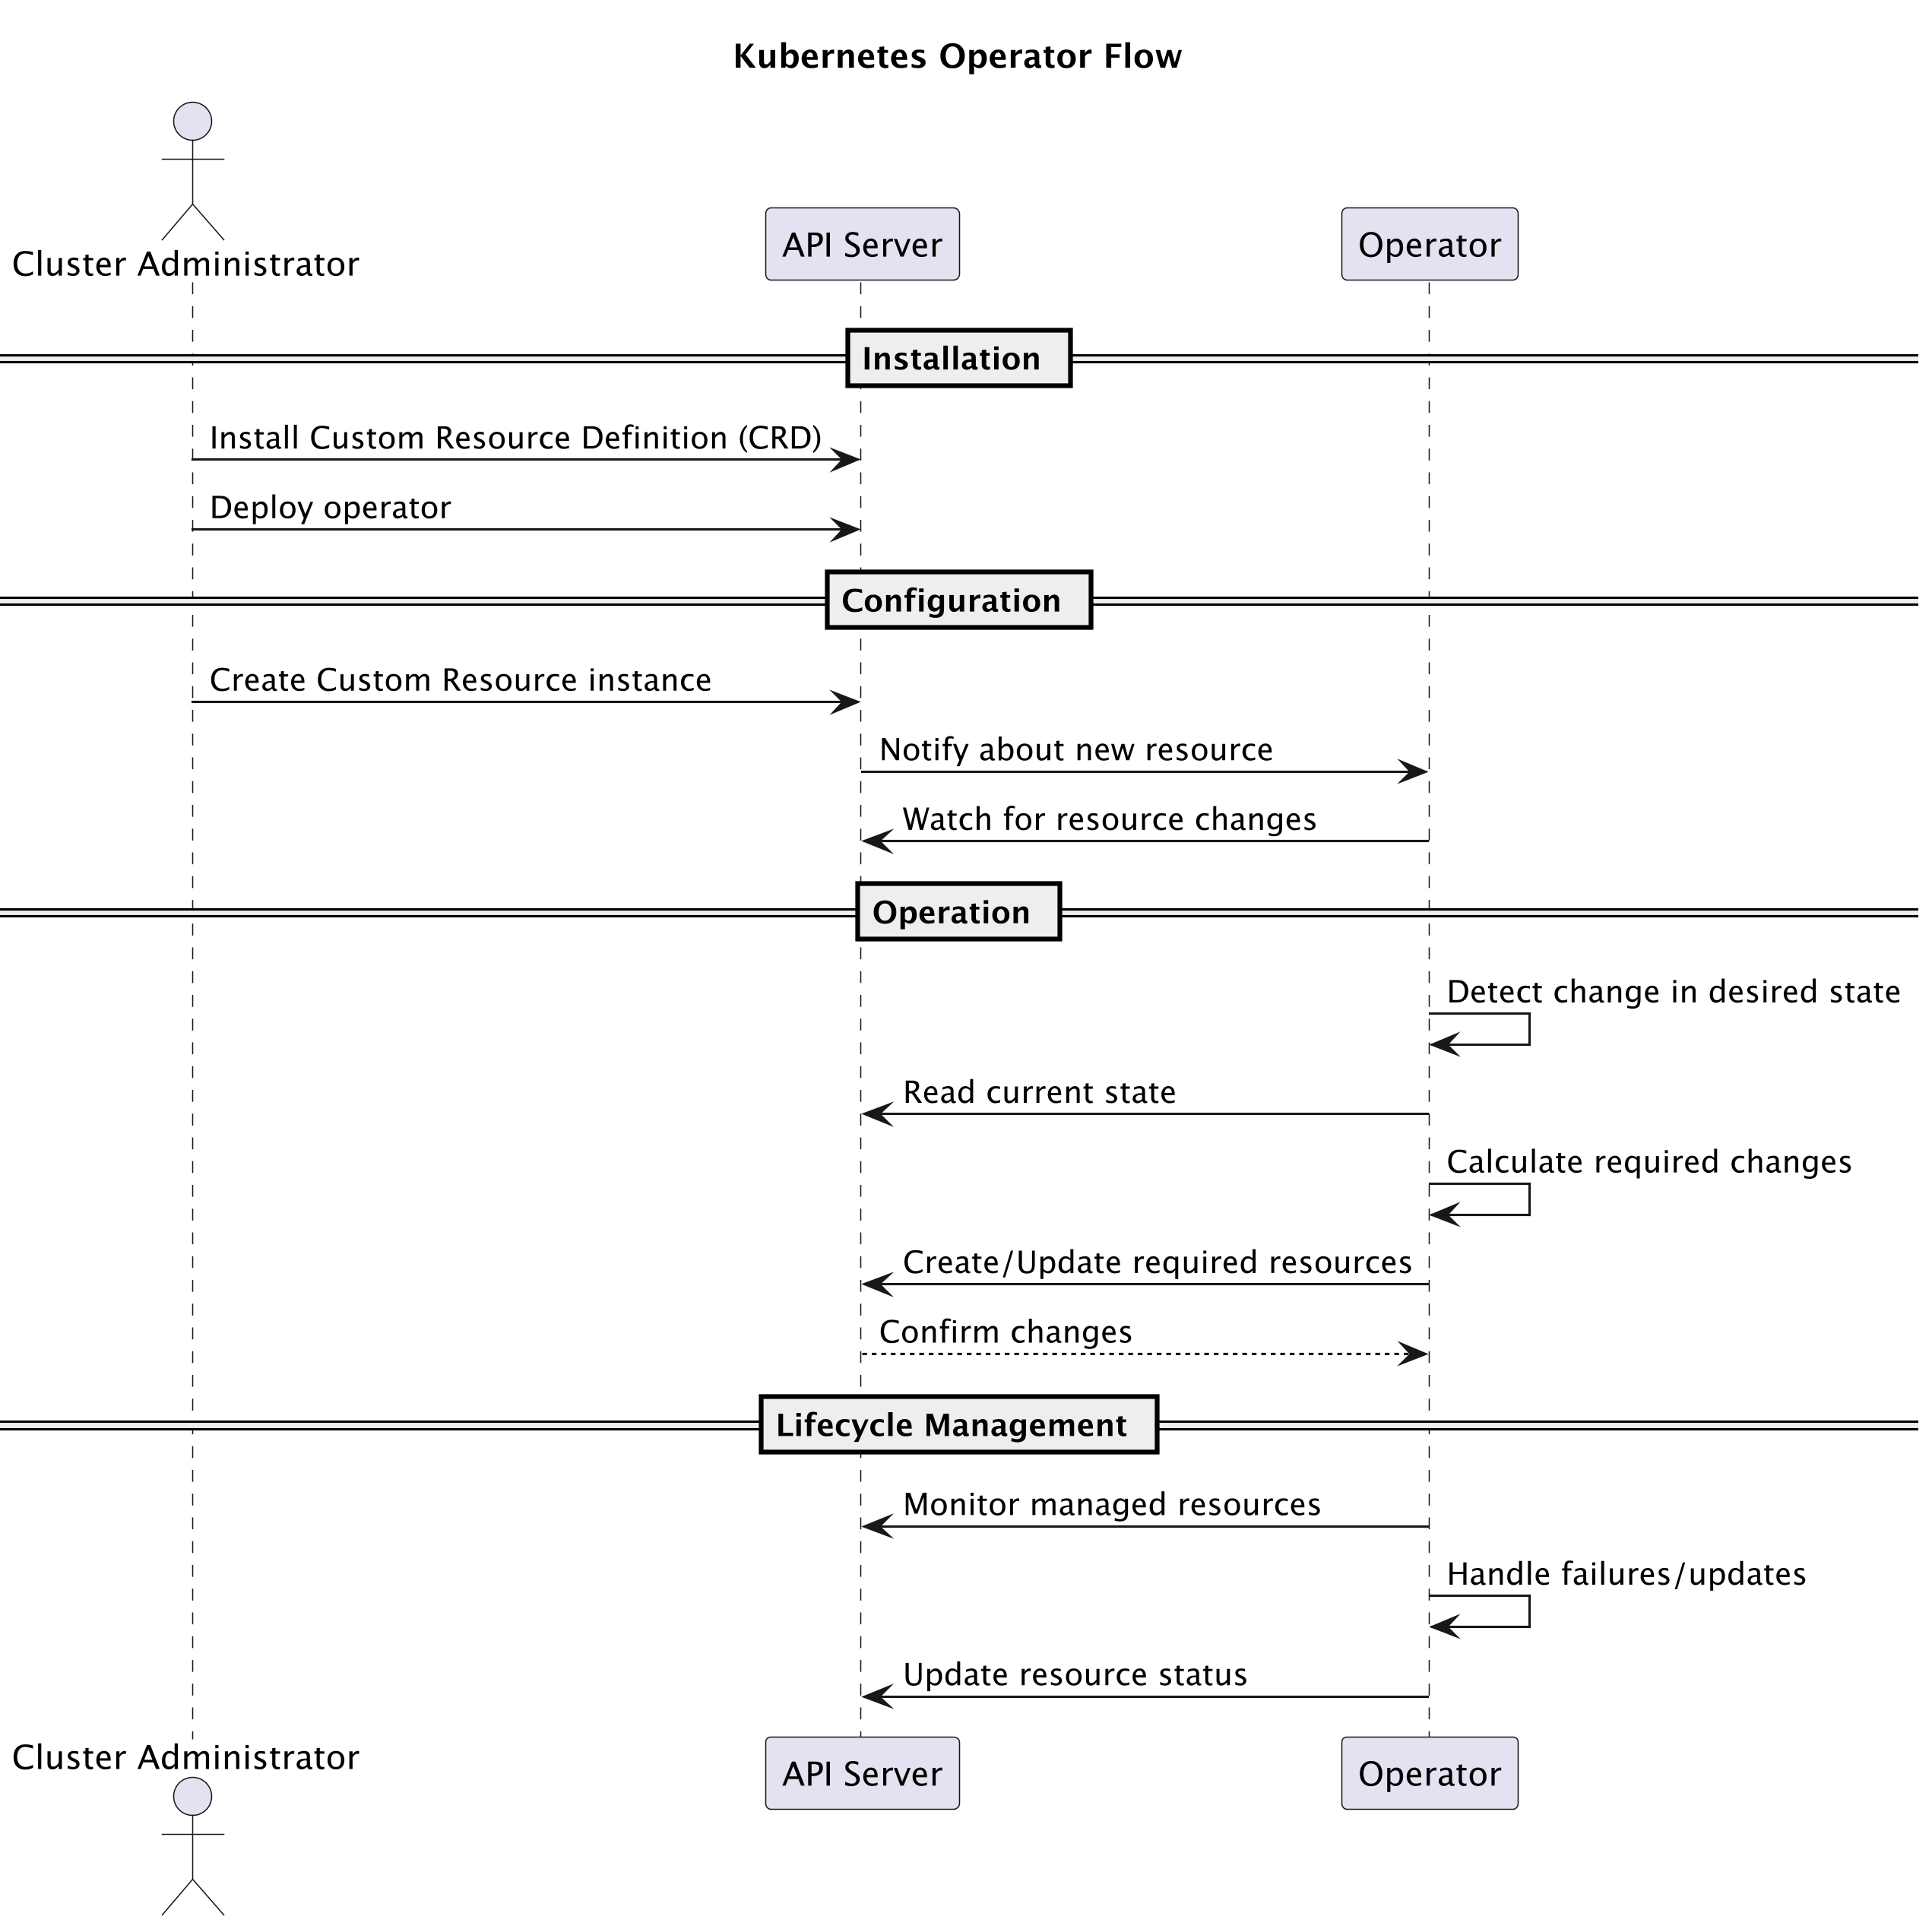
\includegraphics[width=\textwidth]{images/kubernetes_operator_flow}
    \caption{Kubernetes Operator Sequence Diagram demonstrating a reconciliation loop}
    \label{fig:kubernetes-operator-flow}
\end{figure}

The operator pattern enables domain--specific knowledge to be encoded into software that can automatically manage complex applications.
This automation reduces operational overhead and helps maintain consistency across deployments.

\subsection{Go programming language}\label{subsec:go-programming-language}

Go was created in 2007 by a Google team consisting of Robert Griesemer, Rob Pike, and Ken Thompson~\cite{golang}.
Google needed a language that would streamline the creation of large--scale server systems and simplify the software development process in large programming teams.

The first public version of the language was released in 2009.
The language was created with the intention of building scalable server systems that could handle Google's growing infrastructure.
The creators wanted to combine the simplicity of Python with the efficiency of C\@.

The main features of Go are simple syntax, built--in concurrency support, and efficient compilation.
The language offers static typing and automatic memory management.
The Go standard library provides rich support for network operations and concurrent processing.

Go introduces communication channels and goroutines as basic mechanisms for handling concurrency.
Thanks to them, creating parallel programs is much simpler than in other languages.
This is particularly useful in distributed systems.

The Go ecosystem provides tools for automatic code formatting, documentation generation, and dependency management.
Go modules enable versioning and easy code sharing.
The \texttt{go mod} tool automatically manages project dependencies.

Go is a popular choice for creating DevOps tools and cloud systems.
Kubernetes and Docker were written in Go. This language works well in projects requiring high performance and reliability.


\section{Recent Advances in Protein Structure Prediction}

\subsection{Core AlphaFold Developments}

\subsubsection{Improved protein structure prediction using potentials from deep learning (2020)}

Senior et al.
presented AlphaFold (the first version) which uses a deep neural network to predict distances between residue pairs, constructing a potential of mean force that can be optimized by gradient descent to fold the protein~\cite{Senior2020AlphaFold}.
In the CASP13 competition, this method produced high-accuracy structures for 24 out of 43 free-modeling targets, far outperforming other methods.

\subsubsection{Highly accurate protein structure prediction with AlphaFold (2021)}

Jumper et al.
introduced \textbf{AlphaFold2}, a revolution in protein structure prediction.
It regularly achieves atomic accuracy even when no homologous structure is known~\cite{Jumper2021AlphaFold2}.
Validated at CASP14, AlphaFold2's novel architecture (with an attention-based "Evoformer" and end-to-end differentiable structure module) demonstrated accuracy on par with experimental structures in a majority of cases.
This breakthrough showed that computational methods can predict protein 3D structure from sequence alone with unprecedented accuracy.

\subsubsection{Accurate structure prediction of biomolecular interactions with AlphaFold 3 (2024)}

Abramson et al.
unveiled \textbf{AlphaFold 3 (AF3)}, a substantially updated model using a \textbf{diffusion-based architecture} to predict the \textbf{joint structure of complexes} including proteins, nucleic acids, small molecules, and ions~\cite{Abramson2024AlphaFold3}.
AF3 shows markedly improved accuracy over specialized tools: it far outperforms traditional docking for protein–ligand complexes, achieves much higher accuracy on protein–DNA/RNA interactions than prior nucleic-acid-specific predictors, and greatly improves antibody–antigen complex prediction versus AlphaFold-Multimer.
This work demonstrates that a single deep-learning framework can accurately model diverse biomolecular assemblies, heralding a new era of high-accuracy multi-component complex prediction.

\subsection{Conformational Ensemble and Alternative State Prediction}

\subsubsection{Sampling alternative conformational states of transporters and receptors with AlphaFold2 (2022)}

del Alamo et al.
demonstrated that by stochastically subsampling the MSA input, AlphaFold2 can be driven to generate multiple conformations for dynamic proteins~\cite{delAlamo2022AlternativeStates}.
In tests on membrane transporters and GPCRs, this simple MSA-depth reduction yielded accurate models of distinct states (e.g. inward vs.
outward facing), with extreme conformations matching experimental structures (average TM-score ≈0.94).
This study highlighted an underexplored capability of AlphaFold2 to predict conformational ensembles and suggested the need for next-generation AI models that output biophysical state ensembles.

\subsubsection{Structure prediction of alternative protein conformations (2024)}

Bryant \& Noé developed Cfold, a neural network trained on a special "conformational split" of the PDB to predict alternative protein structures~\cite{Bryant2024Cfold}.
By ensuring that conformational variants of the same protein are separated into training vs.
test sets, Cfold can genuinely predict unseen alternative states rather than memorizing them.
The method efficiently explores a protein's conformational landscape and achieved >50\% success in predicting known alternative conformations with high accuracy (TM-score > 0.8).
Cfold demonstrates that neural networks can be adapted to generate biologically relevant conformers, addressing a gap left by AlphaFold2 which was uncertain in predicting truly novel conformations.

\subsubsection{High-throughput prediction of protein conformational distributions with subsampled AlphaFold2 (2024)}

Monteiro da Silva et al.
introduced a method to directly predict the \textbf{relative populations} of protein conformations using AlphaFold2 by subsampling MSAs~\cite{MonteiroSilva2024SubsampledAF2}.
AlphaFold2 typically predicts a single ground-state structure, but here multiple MSA subsets yield an ensemble of states.
When tested against NMR data for two proteins (Abl1 kinase and GM-CSF), the method correctly predicted changes in state populations with >80\% accuracy.
This subsampling strategy was especially effective for qualitatively predicting how mutations or evolution shift conformational landscapes, offering a fast, cost-effective way to estimate conformational distributions for applications in pharmacology and evolution.

\subsection{Physics-Informed and Dynamics-Aware Models}

\subsubsection{Protein Conformation Generation via Force-Guided SE(3) Diffusion Models (2024)}

Wang et al.
introduced ConfDiff, a deep generative model that integrates physical knowledge (forces) into the SE(3)-equivariant diffusion process for protein structure generation~\cite{Wang2024ConfDiff}.
Traditional diffusion models sample protein conformations but can deviate from true equilibrium distributions due to lack of physics.
ConfDiff addresses this by coupling a learned force field with score-based diffusion: the force-guided network steers sampling toward realistic basins, yielding diverse conformations that maintain high fidelity to the native ensemble.
In experiments on 12 fast-folding proteins and BPTI, ConfDiff surpassed prior state-of-the-art methods in capturing native conformational variability. \textit{(Presented at ICML 2024)}

\subsubsection{Simultaneous Modeling of Protein Conformation and Dynamics via Autoregression (2025)}

Shen et al.
proposed \textbf{ConfRover}, the first model to learn \textbf{protein conformational dynamics and structures simultaneously} from MD trajectories~\cite{Shen2025ConfRover}.
ConfRover uses a modular autoregressive design: (i) an encoder adapted from folding models that embeds each time-frame conformation, (ii) a sequence model that captures temporal dependencies between frames, and (iii) an SE(3) diffusion decoder that generates 3D structures for each step.
This enables both time-dependent (trajectory) generation and time-independent sampling of conformations within one framework.
On the large ATLAS MD dataset, ConfRover successfully learned complex motions and could generate realistic trajectories, marking a significant step toward integrating \textit{dynamic behavior} into structure prediction. \textit{(Preprint, May 2025)}

\subsection{Novel Architectural Approaches}

\subsubsection{Structure Language Models for Protein Conformation Generation (2024)}

Lu et al.
proposed a novel framework called \textbf{Structure Language Modeling (SLM)} for efficient generative modeling of protein conformations~\cite{Lu2024SLM}.
Instead of operating purely in 3D coordinate space, SLM first encodes protein structures into a compact latent representation via a discrete VAE, then applies \textbf{conditional language models} to capture sequence-conditioned conformation distributions.
This approach enabled \textbf{20–100× faster} generation of diverse conformations compared to 3D diffusion methods, by exploring ensemble modes in a more tractable latent space.
The authors instantiated SLM with transformer architectures (including a BERT-like model fine-tuned from ESM) and demonstrated its ability to model equilibrium dynamics (e.g. BPTI), conformational changes, and even disordered protein ensembles with high efficiency. \textit{(ICLR 2025 conference paper)}

\subsection{Comprehensive Reviews and Surveys}

\subsubsection{Protein structure prediction via deep learning: an in-depth review (2025)}

Meng et al.
provided a comprehensive review of deep learning techniques for protein structure prediction~\cite{Meng2025DeepLearningReview}.
This article surveys how various architectures – from CNNs and RNNs to GNNs and large language models (LLMs) – have been applied to protein folding.
It discusses advances in databases and resources, evaluates state-of-the-art methods (e.g. AlphaFold2, RoseTTAFold, ESMFold) and their impact on drug discovery, and highlights future challenges.
Key issues identified include the need for improved interpretability of deep models, handling multi-domain and flexible regions, and incorporating dynamics and multi-molecule interactions into predictions.
The review concludes that despite recent breakthroughs, there remains ample room for improving prediction of protein dynamics, complex assemblies, and functional annotations.


\section{Automation of Bioinformatics Workflows}

The scientific literature proposes a range of patterns and tools for managing the infrastructure required for machine learning computations, with particular emphasis on cloud-based solutions and container orchestration.
To understand the current landscape, it is essential to examine both traditional workflow orchestration tools and specific deployment approaches that have emerged in recent years.

\subsection{Traditional Workflow Orchestration Tools}

While specialized bioinformatics platforms provide powerful capabilities, it is important to examine the broader landscape of workflow orchestration tools that have become standard in the field.
These tools, while effective for workflow definition and execution, reveal critical limitations when it comes to infrastructure management -- a gap that operator-based solutions like KubeFold are designed to address.

The bioinformatics community has adopted several workflow management systems, each with distinct characteristics and approaches~\cite{workflows_review_nature}.

\textbf{Nextflow} is a dataflow-based workflow manager that has gained significant popularity in the bioinformatics community.
It provides excellent documentation, supports both Conda environments and container technologies, and offers good integration with cloud platforms.
Nextflow uses a dataflow programming model where processes are connected via their outputs and inputs, enabling automatic parallelization~\cite{nextflow}.
The nf-core community has created a substantial collection of peer-reviewed bioinformatics pipelines, demonstrating the tool's adoption and utility.

\textbf{Snakemake} follows a Make-like approach where users specify output files they want to build, and the system determines the necessary steps to create them.
It is Python-based, making it accessible to researchers familiar with Python, and provides strong support for reproducibility through built-in environment management~\cite{snakemake}.
Snakemake offers excellent support for incremental builds and re-entrancy, allowing workflows to resume from interruption points.

\textbf{Galaxy} provides a web-based platform that abstracts workflow complexity behind a graphical user interface.
It enables researchers without programming expertise to construct and execute complex bioinformatics workflows~\cite{galaxy}.
Galaxy's strength lies in its accessibility and the extensive tool ecosystem, with thousands of pre-configured bioinformatics tools available through its interface.

\textbf{Workflow Description Language (WDL)} and its execution engine \textbf{Cromwell} offer a declarative approach to workflow specification.
WDL provides a standardized way to describe workflows that can be executed across different environments, promoting portability~\cite{wdl_cromwell}.
The approach separates workflow logic from execution details, enabling the same workflow to run on various computing platforms.

\textbf{Common Workflow Language (CWL)} represents an effort to standardize workflow descriptions across different execution engines.
CWL workflows can be executed by multiple workflow runners, providing workflow portability across different computational environments~\cite{cwl}.

Despite their sophistication in workflow orchestration, these traditional tools exhibit significant limitations regarding infrastructure management that highlight the value of operator-based approaches:

\textbf{Manual Infrastructure Provisioning}: While these workflow systems generally require pre-existing computational infrastructure, some tools like Nextflow and Snakemake can integrate with cloud autoscaling services (e.g., AWS Batch, Google Life Sciences API).
However, users must still manually provision core infrastructure, configure networking, set up storage systems, and manage resource allocation before executing workflows.
This places a substantial operational burden on researchers and requires specialized DevOps knowledge.

\textbf{Limited Cloud-Native Integration}: While these tools can execute on cloud platforms, they do not leverage cloud-native technologies like Kubernetes operators for automated infrastructure management.
They treat cloud resources as static infrastructure rather than dynamically managed, declarative resources.

\textbf{Lack of Automated Scaling}: Traditional workflow managers provide limited support for automatic infrastructure scaling in response to workload demands.
Resource allocation is typically configured at deployment time rather than adjusted dynamically based on queue depth or resource utilization.

\textbf{Complex Deployment Requirements}: Deploying these workflow systems in production environments requires significant configuration effort.
Setting up proper cluster managers, configuring security policies, implementing backup strategies, and ensuring high availability demands extensive operational expertise.

\textbf{Separation of Concerns}: These tools excel at workflow orchestration but delegate infrastructure concerns to external systems.
This separation, while following good architectural principles, results in complex operational overhead when researchers need to manage both workflow logic and underlying infrastructure.

\subsection{Foldy}

In the paper \textit{Foldy: a web application for interactive protein structure analysis}, the authors propose a complete deployment of the \textit{Foldy} application on a Kubernetes cluster, using Helm for automated installation and configuration~\cite{foldy,helm}.
The application allows users without advanced bioinformatics knowledge to predict protein structures (AlphaFold), dock ligands (DiffDock, AutoDock Vina), and visualize domains (Pfam).

The application deployment process assumes:
\begin{itemize}
    \item manual provisioning of infrastructure resources: domain name, static IP address, Kubernetes cluster, and database;
    \item automatic deployment of the frontend, backend, and computational workers with a single \texttt{helm install} command;
    \item the ability to run workers locally (on private resources) using a Docker image or bash scripts if Docker is not supported.
\end{itemize}

Foldy uses a task queue mechanism (RedisQueue), and computational workers are scaled dynamically using KEDA and Prometheus.
This approach allows prediction of large protein structures (up to 6000 amino acids) and supports thousands of users~\cite{foldy}.

Table~\ref{tab:foldy-kubefold-comparison} presents a comparison between Foldy and KubeFold across key operational dimensions:

\begin{table}[htbp]
\centering
\caption{Comparison of Foldy and KubeFold platforms}
\label{tab:foldy-kubefold-comparison}
\begin{tabular}{|l|p{5.5cm}|p{5.5cm}|}
\hline
\textbf{Aspect} & \textbf{Foldy} & \textbf{KubeFold} \\
\hline
\textbf{Installation} & 
Requires manual infrastructure provisioning (DNS, cluster, databases), then single \texttt{helm install} command & 
Complex initial setup with Kubernetes operator deployment, but automated resources management afterwards \\
\hline
\textbf{User Interface} & 
Web--based graphical interface & 
YAML configuration files providing declarative infrastructure management \\
\hline
\textbf{Scale} & 
Supports hundreds of users with correctly configured scaling via KEDA & 
Designed for large organizations--automatic resource management and cloud--native scaling \\
\hline
\textbf{Automation Level} & 
Automated workflow execution and scaling, manual infrastructure setup & 
Complete lifecycle automation including job management, artifacts archiving, notifications and cleanup \\
\hline
\textbf{DevOps Requirements} & 
Moderate -- requires initial cluster setup, DNS configuration, and database management & 
High initial setup complexity, minimal ongoing operational overhead due to operator--based automation \\
\hline
\textbf{Target Audience} & 
Researchers and biologists without programming expertise & 
Technical teams and institutions requiring enterprise--grade automation and cloud-native solution \\
\hline
\end{tabular}
\end{table}

\textbf{Limitation:} While Foldy provides a powerful and user-friendly platform, its deployment still requires significant manual configuration and integration effort.
Deployment still involves some infrastructure setup, including configuring DNS, cluster resources, and databases, which can be complex for teams without DevOps experience.
Additionally, monitoring and logging are not provided out-of-the-box and require further setup.
Although some operational tasks can be partially automated, there is no centralized layer managing the full lifecycle of jobs, storage, and infrastructure after deployment.

\subsection{A Comprehensive Cloud Architecture for Machine Learning-enabled Research}

In the paper \textit{A Comprehensive Cloud Architecture for Machine Learning-enabled Research}~\cite{cloud_architecture_for_research}, the authors present a comprehensive architecture deployed at the Texas Advanced Computing Center.
The proposed infrastructure includes:
\begin{itemize}
    \item virtualization using OpenStack (with GPU support via PCI passthrough);
    \item container orchestration using Kubernetes (deployed via Kubespray);
    \item access to GPU-enabled JupyterHub as an interactive interface for researchers;
    \item ability to run long-term services (e.g., inference) via the Tapis Pods API;
    \item orchestration of complex workflows via Tapis Workflows.
\end{itemize}

The architecture enables the execution of machine learning models, data management, and training of models on HPC clusters via an HTTP interface.
Thanks to integration with the Tapis ML Hub, users can search for, deploy, and use pre-trained models from Hugging Face without the need to build them from scratch.

\textbf{Limitation:} Although highly capable, the proposed architecture requires coordination across multiple layers of the stack -- OpenStack, Kubernetes, Tapis services -- which demands specialized knowledge and operational overhead.
GPU provisioning, workflow orchestration, and model deployment are fragmented across various APIs and services, making end-to-end automation challenging for small teams or institutions without dedicated infrastructure engineers.
While powerful in production settings, the architecture lacks a unified interface for researchers to independently manage job submissions, monitoring, and data without DevOps support.

Moreover, Tapis offers an imperative approach to infrastructure management. In contrast, KubeFold offers a declarative approach to infrastructure management, and therefore the user does not need to worry about how to manage infrastructure, only defines the desired state of the system. The KubeFold operator makes decisions on how to achieve that state.

\subsection{Kubeflow: Machine Learning Workflows on Kubernetes}

Kubeflow is an open-source machine learning platform designed to enable deployment, orchestration, and management of ML workflows on Kubernetes~\cite{kubeflow,kubeflow_deployment_study}.
Originally developed by Google as an extension of TensorFlow, Kubeflow has evolved into a comprehensive MLOps platform that supports multiple machine learning frameworks and provides end-to-end ML pipeline capabilities.

The platform consists of several core components:
\begin{itemize}
    \item \textbf{Kubeflow Pipelines} -- provide a platform for building and deploying portable, scalable machine learning workflows based on Docker containers;
    \item \textbf{Notebooks} -- offer web-based development environments (JupyterLab, RStudio, VS Code) running inside Kubernetes pods;
    \item \textbf{Katib} -- provides automated hyperparameter tuning and neural architecture search capabilities;
    \item \textbf{KServe} -- enables model serving with advanced features like canary deployments, autoscaling, and multi-framework support.
\end{itemize}

Kubeflow addresses many challenges in machine learning operations by providing standardized, containerized ML workflows that can run consistently across different cloud providers.
The platform abstracts much of the complexity of Kubernetes while providing researchers with powerful tools for experiment tracking, model versioning, and automated ML.

Pandey et al. conducted a comprehensive study of Kubeflow deployment across different cloud providers (Google Cloud Platform and IBM Cloud), evaluating its performance, ease of setup, and limitations~\cite{kubeflow_deployment_study}.
Their research demonstrated that while Kubeflow provides effective orchestration for ML workflows across cloud environments, it requires substantial setup complexity and ongoing maintenance.

\textbf{Limitations for Batch-Heavy Workloads}: Despite its strengths as the dominant ML framework for Kubernetes, Kubeflow presents several limitations for batch processing tasks with extensive storage requirements, such as AlphaFold:

\begin{itemize}
    \item \textbf{Complex Storage Integration}: Kubeflow pipelines are primarily designed for ephemeral computations with limited persistent storage integration, making it challenging to manage large reference databases (terabytes) efficiently;
    \item \textbf{Infrastructure Management Gap}: While Kubeflow automates ML workflows, it assumes pre-existing infrastructure and requires manual provisioning of storage systems, databases, and cluster resources;
    \item \textbf{Batch Job Limitations}: The platform is optimized for interactive ML development and training rather than long-running batch jobs with complex dependency management;
    \item \textbf{Operational Overhead}: Setup and maintenance require significant DevOps expertise, particularly for complex deployments involving multiple cloud services and storage systems.
\end{itemize}

These limitations highlight why specialized solutions like KubeFold are necessary for computational biology workloads that require comprehensive infrastructure automation, large-scale data management, and batch-oriented processing patterns.

\subsection{BioContainers: Lightweight Automation Alternative}

BioContainers is an open-source, community-driven framework that provides standardized containers for bioinformatics software~\cite{biocontainers}.
Developed as a response to the reproducibility crisis in computational biology, BioContainers offers a lightweight alternative for software deployment and automation in Kubernetes environments.

The framework addresses key challenges in bioinformatics software management:
\begin{itemize}
    \item \textbf{Software Standardization}: Provides consistent containerization guidelines and templates for bioinformatics tools;
    \item \textbf{Reproducibility}: Ensures computational experiments can be reliably repeated across different environments;
    \item \textbf{Dependency Management}: Eliminates conflicts between different software versions and system dependencies;
    \item \textbf{Easy Deployment}: Enables researchers to quickly deploy complex software stacks without manual compilation.
\end{itemize}

The BioContainers architecture consists of:
\begin{itemize}
    \item \textbf{GitHub Organization}: Contains all Dockerfiles, specifications, and tools for container creation and management;
    \item \textbf{Container Registries}: Automated build systems that create and distribute ready-to-use containers;
    \item \textbf{Registry UI}: Web interface for searching, tagging, and accessing available containers;
    \item \textbf{Integration with BioConda}: Automatic container generation from existing Conda packages through "mulled containers".
\end{itemize}

At the time of publication, BioContainers provided over 2,000 containers ready for use, with automatic generation capabilities that leverage existing BioConda recipes.
The project has been integrated with major platforms including Galaxy and PhenoMeNal H2020, demonstrating its adoption in the bioinformatics community.

\textbf{BioContainers as Kubernetes Alternative}: In Kubernetes environments, BioContainers offers several advantages for lightweight automation:

\begin{itemize}
    \item \textbf{Minimal Infrastructure Requirements}: Unlike complex platforms, BioContainers can be deployed with basic Kubernetes resources (Pods, Jobs, Deployments);
    \item \textbf{Tool-Specific Focus}: Each container is optimized for specific bioinformatics tools rather than providing a comprehensive platform;
    \item \textbf{Community Maintenance}: Distributed maintenance model reduces the burden on individual research teams;
    \item \textbf{Standard Compliance}: Follows established containerization best practices and Docker ecosystem standards.
\end{itemize}

\textbf{Comparison with Comprehensive Solutions}: While BioContainers excels at software standardization and basic containerization, it operates at a different abstraction level compared to platforms like KubeFold:

\begin{itemize}
    \item BioContainers focuses on \textit{software packaging} while KubeFold addresses \textit{infrastructure orchestration};
    \item BioContainers requires manual workflow composition while KubeFold provides automated lifecycle management;
    \item BioContainers assumes existing Kubernetes knowledge while KubeFold abstracts infrastructure complexity;
    \item BioContainers provides building blocks while KubeFold offers complete solutions.
\end{itemize}

The complementary nature of these approaches suggests that BioContainers could serve as the foundation for software packaging within more comprehensive automation platforms like KubeFold, combining standardized software containers with automated infrastructure management.

\subsection{The Value of Operator-Based Approaches}

The limitations of traditional workflow orchestration tools demonstrate the value proposition of operator-based solutions like KubeFold.
By integrating workflow management with infrastructure automation through Kubernetes operators, KubeFold addresses the operational gap that exists between workflow definition and infrastructure management.

Where existing solutions require DevOps expertise for proper deployment, KubeFold abstracts infrastructure complexity behind declarative resource definitions.
Where conventional workflow managers treat infrastructure as static, KubeFold provides dynamic resource management that adapts to computational demands.

This integration represents a fundamental shift from treating infrastructure as a prerequisite to treating it as an automatically managed component of the scientific computing platform.

\section{Summary and Identified Gaps}

The review of workflow automation solutions reveals a diverse landscape of tools and platforms, each addressing different aspects of the bioinformatics automation challenge.
From traditional workflow managers like Nextflow and Snakemake, to comprehensive platforms like Kubeflow, to specialized deployments like Foldy, and lightweight alternatives like BioContainers, the field demonstrates growing maturity in addressing reproducibility and scalability concerns.

However, these solutions exhibit different strengths and limitations that highlight distinct gaps in the current ecosystem:

\textbf{Kubeflow}, while serving as the dominant ML framework for Kubernetes, excels at interactive machine learning workflows but struggles with batch-heavy workloads requiring extensive storage management.
Its complexity and infrastructure requirements make it less suitable for computational biology applications like AlphaFold that demand seamless integration of large-scale data management with automated workflow execution.

\textbf{BioContainers} provides excellent software standardization and lightweight deployment options, addressing the reproducibility crisis through consistent containerization.
However, it operates primarily at the software packaging level and requires manual orchestration for complex workflows, leaving infrastructure management to external systems.

\textbf{Foldy} demonstrates the feasibility of user-friendly web interfaces for protein structure prediction but still requires manual infrastructure provisioning and lacks comprehensive lifecycle automation.

The comprehensive cloud architecture by Stubbs et al. showcases powerful multi-layered services but demands significant operational expertise and coordination across multiple technology stacks, making it challenging for smaller research teams.

The key difference between these solutions lies in their level of automation and abstraction: while Foldy provides a ready-to-use web application requiring manual infrastructure setup, and the comprehensive cloud architecture offers powerful but complex multi-layered services, Kubefold focuses on complete automation of the entire lifecycle -- from infrastructure provisioning to job monitoring -- enabling researchers to focus on scientific work rather than operational tasks.

By "Complete automation of the entire lifecycle" we mean managing aspects such as:
\begin{itemize}
  \item downloading databases
  \item deleting databases when they are no longer needed
  \item managing dependencies between different resources in the system (protein conformation prediction job and downloaded database)
  \item notifying users about computation status
  \item archiving artifacts
  \item error handling
\end{itemize} 

The review of existing solutions reveals a significant gap: while powerful cloud architectures and specialized bioinformatics platforms exist, there is a lack of solutions that seamlessly integrate automation, AI algorithms, Kubernetes orchestration, and cloud-native approaches into a unified platform.
This gap represents the primary motivation for developing KubeFold as a comprehensive solution for automated protein structure prediction in cloud environments.
